\chapter{Direct backward ray mapping}
\label{chap:raymapping2}
In Chapter \ref{chap:raymapping1} we introduced an inverse method based on ray mapping reconstruction in PS.
The goal was to calculate the intensity distribution at the target of an optical system. \\ \indent
The idea was to construct a map from the target \point{T} to the source \point{S} using the PS of all the optical lines, which are divided into several regions.  
The method developed in the previous chapter requires that the boundaries of these regions can be determined exactly in every PS. Therefore, also the positive luminance regions were found analytically and the \textit{exact} intensity could be determined. This is only possible for systems formed by straight line segments.\\ \indent
In this chapter we modify the method to systems formed by curved lines. In this case, the boundaries of the regions in PS cannot be determined exactly.
Because of this, we need to apply a numerical procedure. In particular, we develop a method that employs only the PS of the target of the system. 
% Differences
The boundaries are detected applying a bisection procedure in target PS in combination with backward ray tracing. The method is tested for two optical systems: the TIR-collimator and a parabolic reflector. The results are presented in Section \ref{sec:TIR} and \ref{sec:PR}, respectively.
\section{Bisection method and backward ray tracing}\label{sec:raymapping_explanation}
The purpose of this section is to present the direct backward ray mapping method valid for systems formed by curved lines. 
Given a partition $P: -1 = \variabile{p}^0<\variabile{p}^1<\cdots<\variabile{p}^{\nbin}=1$ of the interval $[-1,1]$ with $\nbin$ the number of bins in the partitioning, the intensity in target PS is given by Equation (\ref{eta2}) for every $\dir{}{}\in P$.
Therefore, the problem reduces to calculating the coordinates 
$\variabile{q}^{\textrm{\,min}}(\Pi, \variabile{p})$ and $\variabile{q}^{\textrm{\,max}}(\Pi, \variabile{p})$ of the rays on $\partial$\set{R}{}{}$(\Pi)$ for every path $\Pi$. 
\\ \indent 
We indicate with $(\variabile{q}^{\,\textrm{a}}, \variabile{p})= (-\variabile{b}, \variabile{p})$ and $(\variabile{q}^{\,\textrm{b}}, \variabile{p}) = (\variabile{b}, \variabile{p})$ the coordinates of the end points of \set{T}{}{} along direction $\variabile{p}$. These points are associated to two rays in PS. Consider the corresponding position coordinate $(\variabile{x}^{\textrm{a}}, \variabile{z}^{\textrm{a}})$ and $(\variabile{x}^{\textrm{b}}, \variabile{z}^{\textrm{b}})$ and angular coordinates $\optangle^{\variabile{a}}$ and $\optangle^{\variabile{b}}$ of the ray in real space, where $\variabile{x}^{\textrm{a}} = \variabile{q}^{\textrm{a}}$, $\variabile{x}^{\textrm{b}} = \variabile{q}^{\textrm{b}}$, $\variabile{z}^{\textrm{a}} = \variabile{z}^{\textrm{b}} = \variabile{h}$ where $\variabile{h}$ is the height of the target and $\optangle^{\textrm{a}}= \optangle^{\textrm{b}}=\variabile{p}$ refers to the emitted ray. Next, the rays parametrizations $\vect{r}_{\textrm{a}}(s)$ and $\vect{r}_{\textrm{b}}(s)$ are determined according to (\ref{parametrization}).
We remind the reader that, in real space, the coordinates of each ray on line $\lineai\neq \nline$ are indicated with $(\variabile{x}_{\lineai}, \variabile{z}_{\lineai})$ and $\optangle_{\lineai}$ where $(\variabile{x}_{\lineai}, \variabile{z}_{\lineai})$ are the coordinate of the intersection point between the ray and line $\lineai$ and $\optangle_{\lineai}$ is the direction of the incident ray with respect to the \textit{optical axis}. 
%We remind the reader that in the previous chapter we indicated with $(\pos{t,}{\lineai},\dir{t,}{\lineai})$ the coordinates of the rays in target PS \set{T}{\lineai}{} in where the directions coordinates were expressed with respect to the \textit{normal} of line $\lineai$. Note that $\pos{\lineai}{}=\pos{t,}{\lineai}$ while $\dir{\lineai}{}\neq\dir{t,}{\lineai}$. We introduce the notation $(\pos{\lineai}{}^{\textrm{a}}, \dir{\lineai}{}^{\textrm{a}})$ for the coordinates of ray $\vect{r}_{\textrm{a}}(s)$ on line $\lineai$.\\ \indent 
The procedure starts with intensity $I(\variabile{p})=0$ and the end points $(\variabile{q}^{\,\textrm{a}}, \variabile{p})= (-\variabile{b}, \variabile{p})$ and $(\variabile{q}^{\,\textrm{b}}, \variabile{p}) = (\variabile{b}, \variabile{p})$. Since the boundaries of the regions in all the phase spaces are unknown, to determine from which line $\vect{r}_{\textrm{a}}$ and $\vect{r}_{\textrm{b}}$ are emitted we apply backward ray tracing. We denote with $\nline$ the index of the target (line $\nline$) and with $\lineaj\in\{1,\cdots, \nline-1\}$ and $\lineak\in\{1,\cdots, \nline-1\}$ the lines from which the rays with parametrization $\vect{r}_{\textrm{a}}(s)$ and $\vect{r}_{\textrm{b}}(s)$ are emitted, respectively. $\Pi^\textrm{a} = (\lineaj, \nline)$ and $\Pi^\textrm{b} = (\lineak,\nline)$ are the last part of the paths followed by the two rays $\vect{r}_{\textrm{a}}$ and $\vect{r}_{\textrm{b}}$, respectively, and $(\variabile{q}^{\textrm{a}}, \variabile{p})\in\partial$\set{R}{}{}$(\Pi^{\textrm{a}})$ and $(\variabile{q}^{\textrm{b}}, \variabile{p})\in\partial$\set{R}{}{}$(\Pi^{\textrm{b}})$. At this stage we know whether the two rays are emitted from the same line or not. \\ 
\begin{figure}[h]
  \begin{center}
  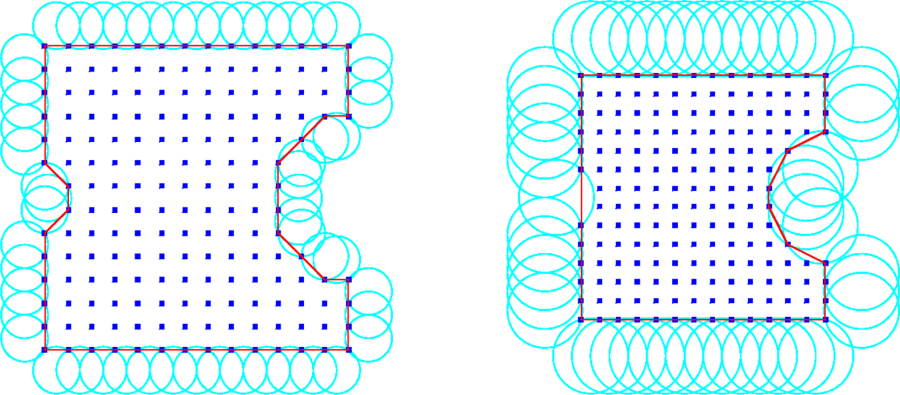
\includegraphics[width=0.7\textwidth]{figures/alpha_shape2D.png}
  \end{center}
  \caption{\textbf{Bisection in target PS \set{T}{}{}.} Algorithm \ref{alg:bisection} is run for the interval $[\variabile{q}^{\textrm{a}}, \variabile{q}^{\textrm{b}}]$ along direction $\variabile{p}=0$. The coordinates $\variabile{q}^{\textrm{c}}$ and $\variabile{q}^{\textrm{d}}$ are found such that 
$|\variabile{q}^{\textrm{c}}-\variabile{q}^{\textrm{d}}|<\textrm{tol}$. $\Pi^{\textrm{c}}= \Pi^{\textrm{a}}$ and $\Pi^{\textrm{d}}\neq \Pi^{\textrm{a}}$.}
\label{fig:bisec}
 \end{figure}
 Ciao \ref{fig:bisec}
